\documentclass[11pt, a4paper]{book}

\usepackage[a4paper, left=1.27cm,top=1.27cm,right =1.27cm, bottom = 1.4cm]{geometry}
%\setlength{\parindent}{0cm}

\usepackage[dutch]{babel}
\usepackage{mathtools}
\usepackage{upgreek}


\usepackage{graphicx}
\graphicspath{{figures/}}

\begin{document}
    
    \tableofcontents

    \chapter{Krachten, momenten, spanningne en rekken}

    \section{STATICA EN EVENWICHT VAN CONSTRUCTIES}

        \subsection{Types ondersteuningen}

            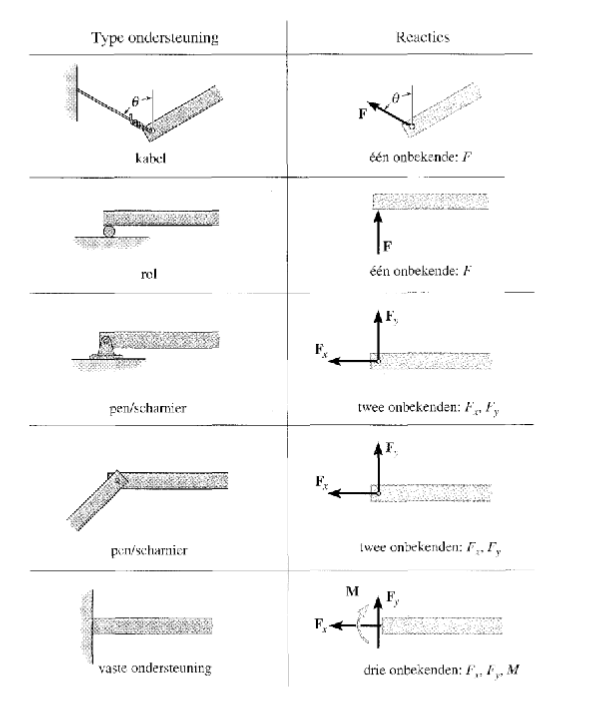
\includegraphics[scale=0.5]{ondersteuningen.png}

        \subsection{Evenwicht van een constructie}

            \begin{align*}
                &\sum\mathbf{F} = 0\\
                &\sum\mathbf{M}_O = 0\\
            \end{align*}
    
    \section{INTUÏtIEF BEGRIP VAN SPANNINGEN EN REKKEN}

        \begin{align*}
            &\upsigma = \frac{F}{A_0}\\
            &\upvarepsilon = \frac{\Delta L}{L_0}\\
            &\upsigma = E\cdot \upvarepsilon
        \end{align*}

    \section{SPANNINGEN}
        
        \subsection{Definitie}

            De spanningsvector
            \begin{equation}
                \vec{\upphi}^{(n)} = \lim_{\Delta A \rightarrow 0} \frac{\Delta F}{\Delta A}
                \label{spanningsvector}
            \end{equation}
            De normaalspanning
            \begin{equation}
                \upsigma = \lim_{\Delta A \rightarrow 0} \frac{\Delta F_n}{\Delta A}
                \label{normaalspanning}
            \end{equation}
            De schuifspanning
            \begin{equation}
                \uptau = \lim_{\Delta A \rightarrow 0} \frac{\Delta F_t}{\Delta A}
                \label{schuifspanning}
            \end{equation}
            De spanningstensor
            \begin{equation}
                [\sigma] = \left[\begin{matrix}
                    \upsigma_{xx} & \uptau_{xy} & \uptau_{xz} \\
                    \uptau_{yx} & \upsigma_{yy} & \uptau_{yz} \\
                    \uptau_{zx} & \uptau_{zy} & \upsigma_{zz}
                \end{matrix}\right]
                \label{spanningstensor}
            \end{equation}

        \subsection{Verband tussen spanningsvector $\vec{\upphi}^{(n)}$ en spanningstensor $[\upsigma]$}
            
            Het verband tussen de spanningsvector en spanningstensor
            \begin{equation}
                \upsigma_{ij}\cdot n_i = \upphi_j^{(n)} \;\;\; (i,j=x,y,z)
                \label{spannigsvector_tensor}
            \end{equation}

        \subsection{Vergelijkingen van het evenwicht}

            De vergelijkingen van het evenwicht
            \begin{align}
                &\frac{\partial \upsigma_{xx}}{\partial x} + \frac{\partial \uptau_{yx}}{\partial y} + \frac{\partial \uptau_{zx}}{\partial z} + F_x = 0\nonumber\\
                &\frac{\partial \uptau_{xy}}{\partial x} + \frac{\partial \upsigma_{yy}}{\partial y} + \frac{\partial \uptau_{zy}}{\partial z} + F_y = 0 \\
                &\frac{\partial \uptau_{xz}}{\partial x} + \frac{\partial \uptau_{yz}}{\partial y} + \frac{\partial \upsigma_{zz}}{\partial z} + F_z = 0\nonumber\\
                \label{vergelijkingen_van_het_evenwicht}
            \end{align}
            Wet van de wederkerigheid der schuifspanningen
            \begin{align}
                &\uptau_{xy} = \uptau_{yx}\\
                &\uptau_{xz} = \uptau_{zx}\\
                &\uptau_{yz} = \uptau_{zy}\\
            \end{align}

        \subsection{Transformatie van coördinaten en hoofdrichtingen}

            \begin{equation}
                [\upsigma'] = [a]\cdot[\upsigma)\cdot[a]^{\top}
                \label{spanningstransformatie}
            \end{equation}
            met
            \begin{equation}
                a_{rk} = \vec{e}'_r\cdot\vec{e}_k \;\;\; r,k=x,y,z
                \label{Transformatiematrixelementen}
            \end{equation}
            
        \subsection{Kromlijnige coördinaten}
            
            \subsubsection{Cilindercoördinaten}

                De spanningstensor
                \begin{equation}
                    [\upsigma] = \left[\begin{matrix}
                        \upsigma_{rr} & \uptau_{x\theta} & \uptau_{rz} \\
                        \uptau_{r\theta} & \upsigma_{\theta \theta} & \uptau_{\theta z} \\
                        \uptau_{rz} & \uptau_{\theta z} & \upsigma_{zz}
                    \end{matrix}\right]
                \end{equation}

    \section{Rekken}

        \subsection{Eendimensionale lengteverandering}            

    \chapter{Tweedimensionel problemen}

\end{document}